\documentclass[titlepage,a4paper]{article} 
\usepackage{verbatim}
\usepackage[T1]{fontenc}
\usepackage[utf8]{inputenc}
\usepackage[brazil]{babel}
\usepackage{hyperref}
\usepackage{rotating}
\usepackage{listings}
\usepackage{color}
\usepackage{listings}
\usepackage{float}
\usepackage{amsmath, amsthm, amssymb}
\hypersetup{colorlinks=true,%
	citecolor=red,%
	linkcolor=red,%
	urlcolor=blue,%
	pdftex}

\definecolor{Brown}{cmyk}{0,0.81,1,0.60}
\definecolor{OliveGreen}{cmyk}{0.64,0,0.95,0.40}
\definecolor{CadetBlue}{cmyk}{0.62,0.57,0.23,0}

\newcommand{\opensource}{\textit{open source}}
\newcommand{\software}{\textit{software}}
\newcommand{\calopsita}{Calopsita}


\title{\calopsita: Um sistema gerenciador de projetos que utilizam metodologias ágeis}
\author{Cauê Haucke Porta Guerra\\Cecilia Fernandes\\Lucas Cavalcanti dos Santos\\ \\Orientador: Prof. Dr. Alfredo Goldman}

\begin{document}
	
\lstset{language=Java,frame=ltrb,framesep=5pt,basicstyle=\footnotesize,
  keywordstyle=\ttfamily\color{OliveGreen},
 identifierstyle=\ttfamily\color{CadetBlue}\bfseries, 
 commentstyle=\color{Brown},
 stringstyle=\ttfamily,
 showstringspaces=false,
 showspaces=false,
 tabsize=2}

\maketitle

\begin{description} 
\item{\textbf{Alunos:}\\Cauê Haucke Porta Guerra\\Cecilia Fernandes\\Lucas Cavalcanti dos Santos}
\item{\textbf{Supervisor:}\\Prof. Dr. Alfredo Goldman}
\item{\textbf{Colaboradores:}\\Mariana V. Bravo\\Hugo Corbucci\\Paulo E. de Azevedo Silveira\\Guilherme de Azevedo Silveira}
\end{description}

\section{Introdução}
O \calopsita é um projeto que nasceu da necessidade de se trabalhar e gerenciar diferentes projetos ágeis, cada um com suas particularidades. Em especial, surgiu da necessidade de se trabalhar com equipes distribuidas em projetos ágeis. 

Essa necessidade ficou evidente em projetos de consultoria da empresa na qual os três idealizadores do \calopsita trabalham: o Product Owner dos projetos é externo, mas ainda tem que escrever cartões de estórias, priorizá-los e acompanhar o desenvolvimento da iteração, ainda que à distância.

Não é intenção do \calopsita substituir métricas coladas em paredes e quadros brancos, mas sim prover uma ferramenta que permita o desenvolvimento ágil distribuido -- tanto comercial quanto \opensource.  

Esse objetivo convergia para os mestrados de dois amigos, Hugo Corbucci e Mariana Bravo, então resolvemos convidá-los para serem nossos clientes de projeto -- convite esse que foi aceito prontamente. Além deles, contamos com o apoio do nosso orientador, que acompanhava o andamento do projeto pela lista de discussões e conversas esporádicas, e com alguns amigos da Caelum, que foram de fundamental importância nas discussões sobre a arquitetura do sistema e que, mais tarde, também tornaram-se clientes e passaram a pedir por novas funcionalidades e reportar bugs. 

Já desde abril, o sistema é usado para gerenciar seu próprio desenvolvimento e, hoje, auxilia no desenvolvimento de vários outros projetos, tanto da Caelum como pessoais.

Nesse trabalho, temos três temas principais relacionados ao \calopsita. Primeiramente, o processo de desenvolvimento, isto é, quais foram os métodos ágeis adotados para gerenciamento do sistema, a importante interação com clientes e a infraestrutura que viabilizou o crescimento e estabilidade do sistema. 

Em seguida, veremos uma parte mais técnica que explica as inovações presentes no código do \calopsita, de onde elas vieram, o que as motivou e nossas impressões sobre esses avanços no estado da arte do mercado Java.

Finalmente, falaremos do sistema produzido, comparando-o com outras ferramentas de proposta similar já existentes, \opensource e comerciais, do feedback dos clientes atuais e dos passos futuros a serem implementados.

\section{Motivação e público alvo}

A motivação maior de se contruir um sistema para gerenciamento de projetos ágeis e seu público alvo estão intimamente relacionados. 

Em aplicações comerciais, uma das maiores reclamações com relação à adoção de métodos ágeis é de que é impossível ter um cliente presente a todo tempo, por mais acessível que ele esteja. Se houvesse uma forma de o cliente se manter informado com o andamento do seu \software e priorizar os próximos cartões online, ajudaria.

E esse não é o único problema que o desenvolvimento ágil enfrenta hoje. Equipes distribuidas estão cada vez mais comuns -- desenvolvedores que pareiam em código e conversam através da telecolaboração de que tem falado Frederich Brooks, e será um dos assuntos de seu próximo livro~\cite{brooks}. Lidar com equipes distribuidas requer uma centralização das informações do projeto acessível de qualquer lugar do mundo.

Um outro grande exemplo da necessidade de tabalhar num mesmo projeto com pessoas de qualquer parte do mundo é o desenvolvimento \opensource. Sistemas de tickets são muito usados nesse nicho, mas muitos deles deixam a desejar ou são complexos de mais para se entender.

Para tantos públicos, a limitação a uma determinada metodologia, seus métodos e métricas não é viável. Gostaríamos de poder personalizar o Calopsita de acordo com as necessidades dos que utilizam e, assim, desde o começo, houve uma grande atenção em não focar numa metodologia apenas -- que é o que o mercado já oferece hoje.

Embora o Calopsita seja mais uma ferramenta, sua intenção é ser um facilitador das interações entre os indivíduos de um determinado projeto, indo de acordo com um dos valores do Manifesto Ágil~\cite{manifesto}:

``Individuals and interactions over processes and tool''

Nessa linha, partimos de uma idéia de desenvolver um sistema adaptável e flexível, que se adapte às necessidades de cada equipe, independente dos métodos adotados e que seja capaz de unir uma equipe distribuida.



\section{Desenvolvimento}

Já desde o início de janeiro, a proposta inicial do \calopsita foi montada. Durante o mês de janeiro, estudamos tecnologias que poderiam ser interessantes no desenvolvimento do projeto e conseguimos o apoio do professor Alfredo Goldman, que aceitou nos orientar, da Caelum, que nos cedeu horas do trabalho e dos mestrandos Mariana Bravo e Hugo Corbucci, nossos clientes eleitos.

Também desde então temos o grupo de discussões~\footnote{http://groups.google.com/group/\calopsita-development} e um repositório no GitHub para o projeto~\footnote{http://github.com/caelum/\calopsita}. Esse repositório foi movido durante o desenvolvimento, mas seu histórico completo se manteve. Abaixo, um gráfico de número de linhas enviadas ao repositório no decorrer do ano ilustra a distribuição do trabalho de código durante o ano.

\begin{figure}[H]
  \centering
  \fbox{
    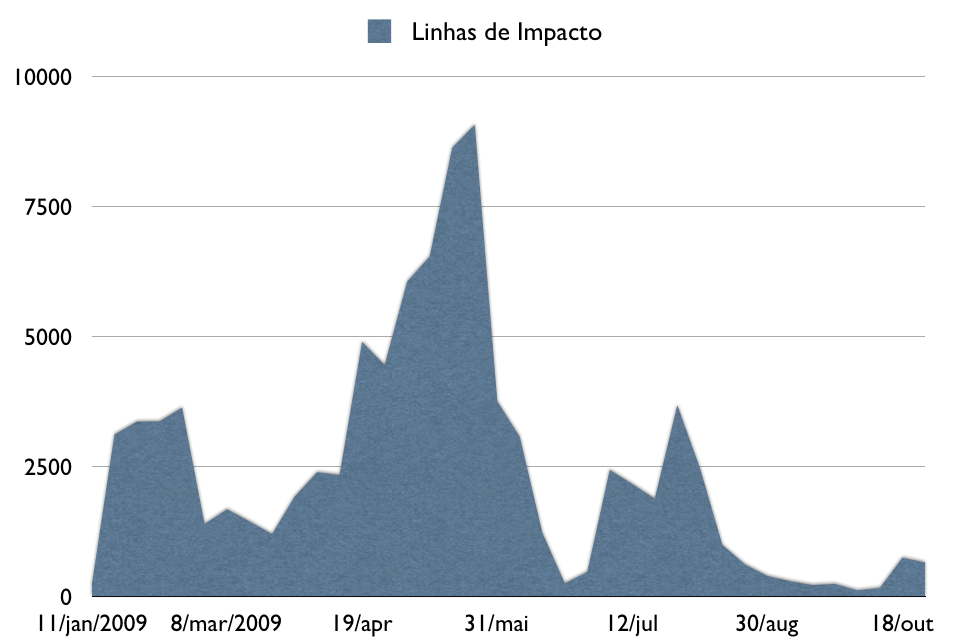
\includegraphics[width=110mm]{images/impacto.png}
  }
  \caption{Linhas de impacto - GitHub}
\end{figure}

Esses dados foram colhidos do gráfico de impacto do GitHub e as divisões de linhas por desenvolvedor foram removidas porque, como adotamos programação pareada na maioria do tempo, ele não necessariamente representa a cota de cada desenvolvedor no projeto.

Nota-se dessa imagem um pico de linhas de código enviadas ao repositório no mês de maio, mês seguinte a começarmos a gerenciar o próprio \calopsita usando a parte que já estava pronta do projeto. Contudo, houve trabalho de janeiro até o momento atual, com uma considerável queda em setembro para que focássemos nessa monografia.

\subsection{Abordagem ágil}

Por tratar-se de um projeto de médio porte, seria indicado optar por alguma metodologia de gerenciamento de \software. Métodos tradicionais nem sequer foram considerados. Há algumas razões para isso.

Primeiramente porque, buscando informações históricas sobre o modelo \textit{Waterfall}, descobrimos que mesmo o artigo~\cite{waterfall} que primeiro descreveu o modelo avisava que sua implementação é quase utópica e propensa a falhas.

``I believe in this concept, but the implementation described above is risky and invites failure.''

Mais do que isso, o autor, já em 1970 sugeria que o desenvolvimento iterativo é mais apropriado para o desenvolvimento de projetos de \software. Isso apenas aumenta nossa consternação com relação ao que se vê no mercado de trabalho ainda hoje -- diversas empresas que clamam usar RUP~\cite{rup} ignoram sua parte mais importante, o desenvolvimento iterativo.

Em segundo lugar, métodos tradicionais prezam pelo conhecido "Big Design Up Front" 

 

\subsection{metodos}

Durante o desenvolvimento do \calopsita, utilizamos alguns métodos presentes em XP e Scrum que melhor funcionavam para nosso time. Aliás, acreditamos que não exista uma única maneira de desenvolver \software de maneira ágil e esse é um dos fatores que motivaram a criação do \calopsita: precisávamos de uma ferramenta que se adequasse às nossas necessidades. Nosso time resolveu adotar como ferramenta de tracking do projeto o KanBan:

\begin{figure}[H]
  \centering
  \fbox{
    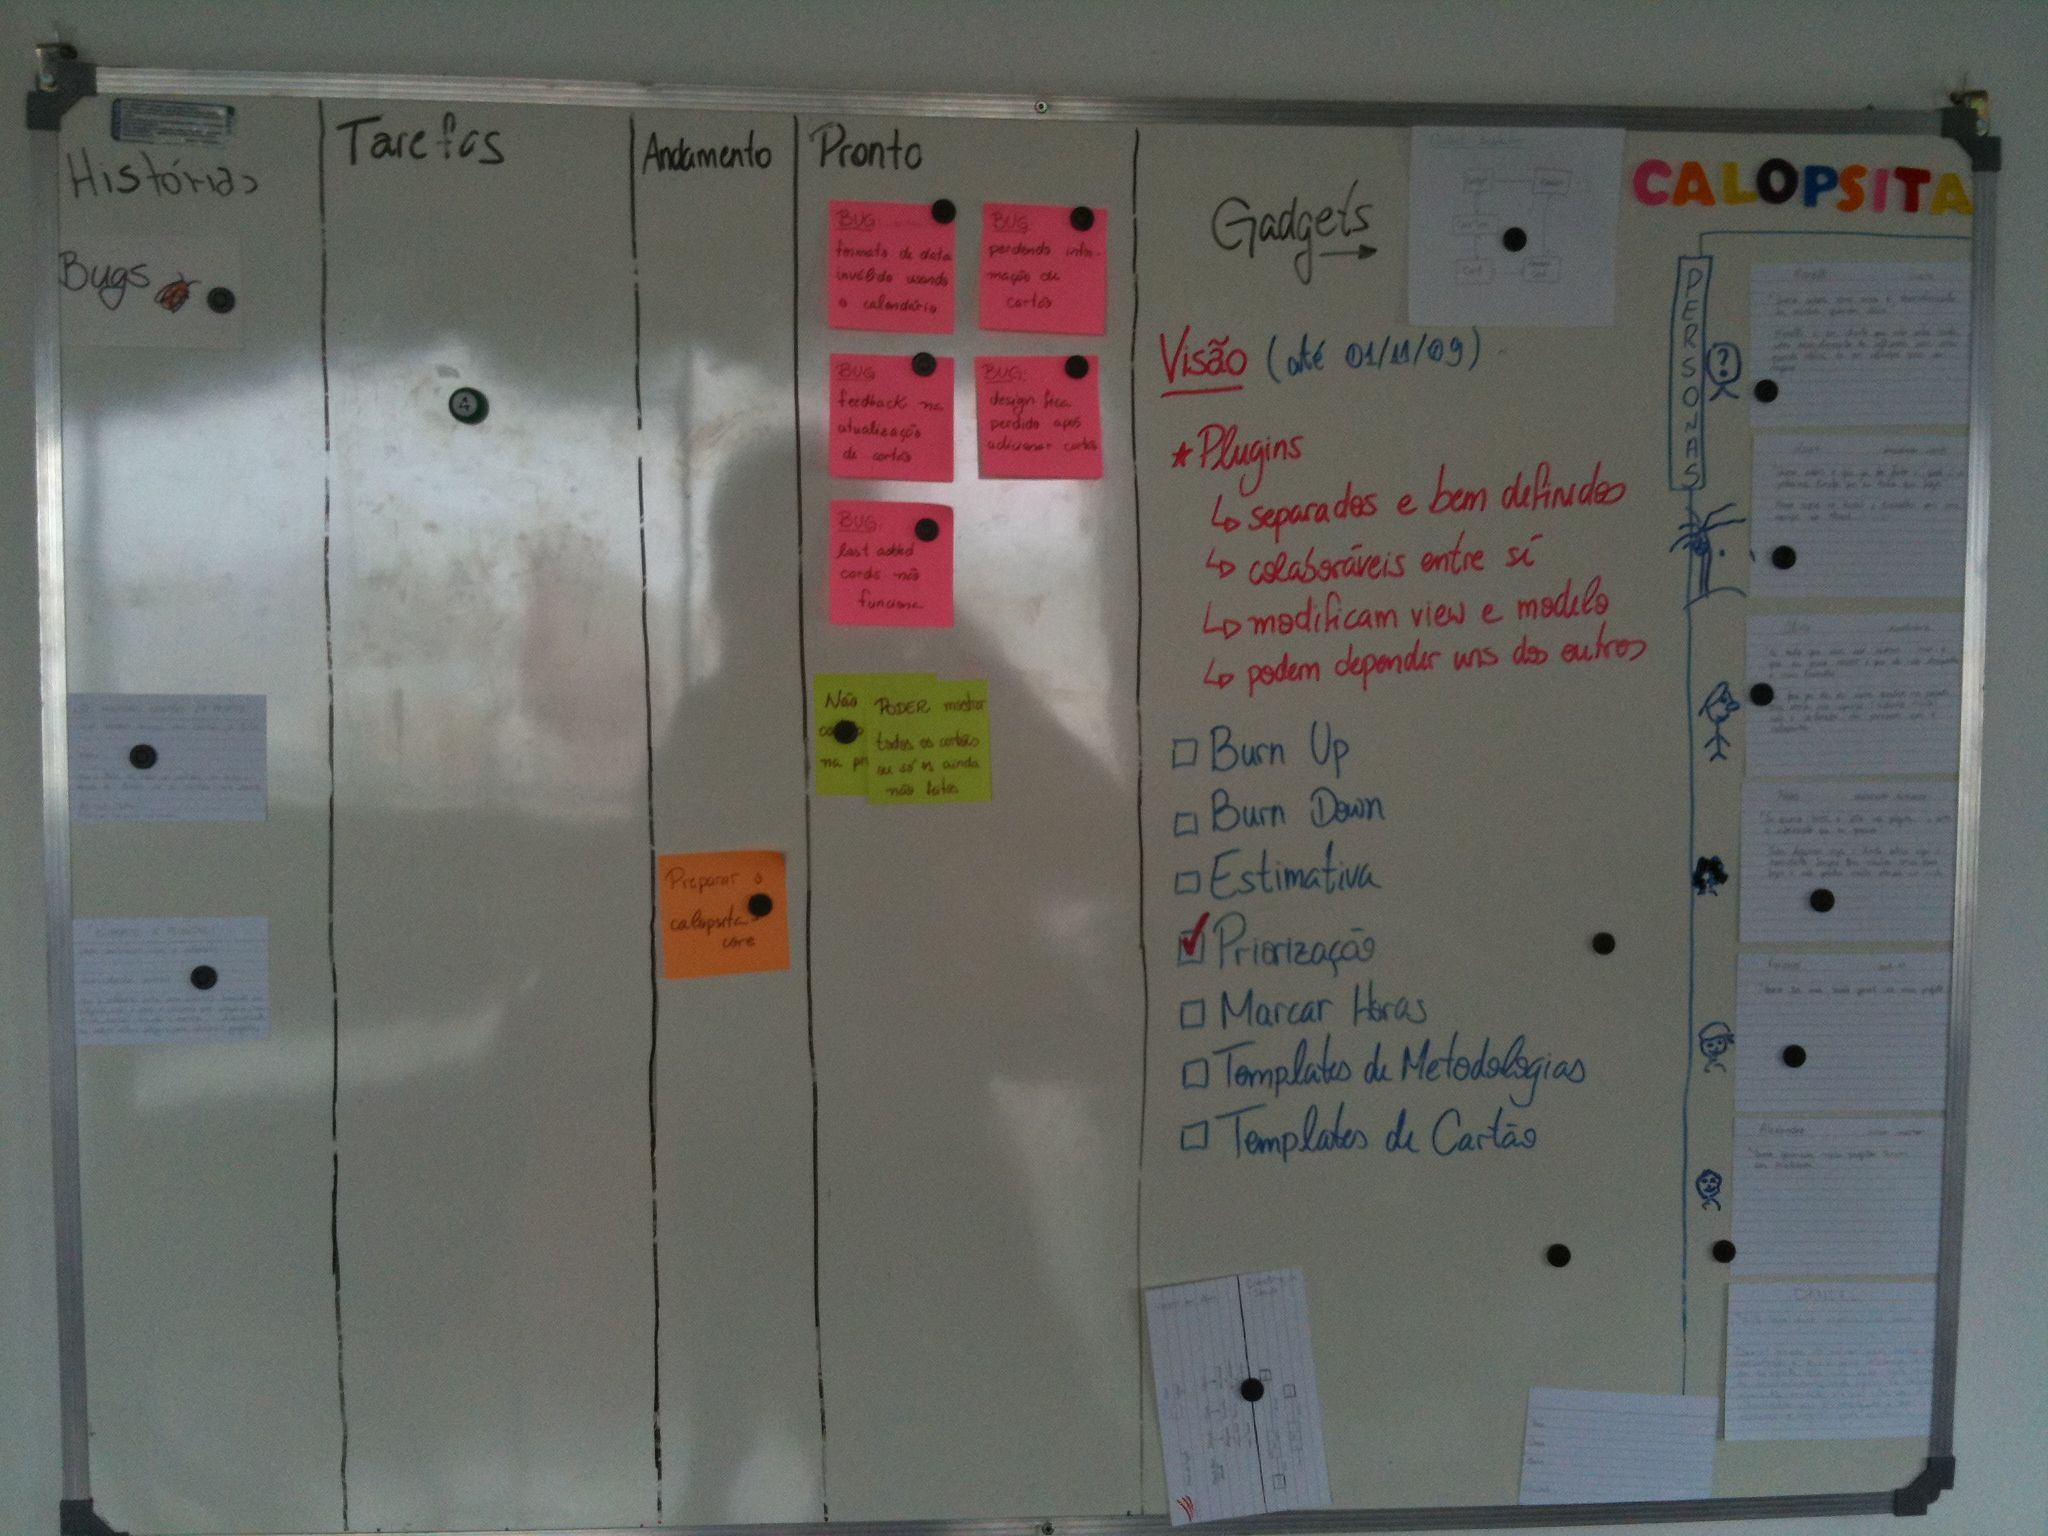
\includegraphics[width=110mm]{images/calopsita-kanban.jpg}
  }
  \caption{KanBan do \calopsita}
\end{figure}

Para mantermos a qualidade de nosso código, utilizamos desde o começo do projeto um servidor de integração contínua~\cite{ci}, o CruiseControl.rb~\footnote{http://cruisecontrolrb.thoughtworks.com/}. Esse servidor é capaz de **pingar** o repositório de código de tempos em tempos verificando por mudançar no código, e uma vez detectada alguma alteração, ele baixa o novo código, compila e roda seus testes de forma automática. Se durante esse processo, qualquer um dos testes falha, um email é disparado para toda a equipe, garantido que o bug introduzido seja corrigido o mais rapidamente possível.

\begin{figure}[H]
  \centering
  \fbox{
    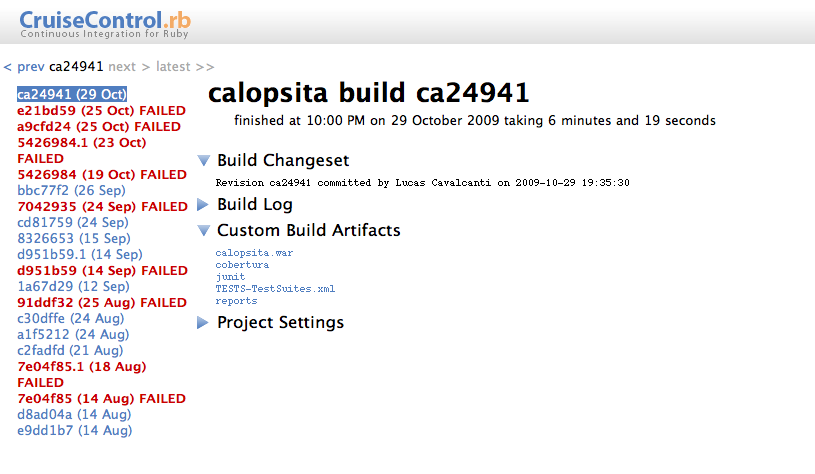
\includegraphics[width=110mm]{images/cruisecontrol-calopsita.png}
  }
  \caption{Cruisecontrol.rb do \calopsita}
\end{figure}

Clientes reais e distribuidos
Muito pareamento
Kanban + \calopsita
Usamos XP e ?????
TDD e Integração Contínua


\section{Código}
Todo o código do \calopsita está hospedado no GitHub, local onde também pode ser visualizado todo o histórico e atividades do projeto desde sua concepção.

Antes de iniciar o desenvolvimento do \calopsita, foi discutido quais seriam as escolhas de linguagens e frameworks a 
serem utilizados. As opções eram: Ruby on Rails ou Java com VRaptor. Como a maioria da equipe era mais familiar com Java 
do que com Ruby, a escolha foi pelo Java com VRaptor.

\subsection{BDD} \label{bdd}
Desde o começo resolvemos adotar boas práticas de desenvolvimento, como {\it Behavior Driven Development} (BDD) \cite{bdd}, 
refatoração constante e programação pareada. Principalmente para usar BDD precisávamos de ferramentas que nos 
ajudassem a escrever testes mais expressivos e legíveis. No mundo do Ruby on Rails essa prática já está bastante 
difundida, então existem várias ferramentas de teste como o RSpec~\footnote{http://rspec.info/} e o
Cucumber~\footnote{http://cukes.info/}, além da linguagem ser dinâmica e possibilitar a escrita de DSLs e interfaces
fluentes~\cite{dsl} de uma maneira bastante direta. Em Java a prática de BDD ainda não está muito forte, então não existem
ferramentas muito avançadas, além da linguagem ser estática e burocrática, que torna o desenvolvimento de tais ferramentas 
muito mais difícil. Mesmo assim, foram pesquisadas as alternativas:

\begin{itemize}
	\item{JBehave~\footnote{http://jbehave.org/} - funciona associando um arquivo texto a um código Java. No arquivo texto fica 
	a descrição da funcionalidade, tal como seria escrita num cartão de estória. Foi descartado por causa da sua sintaxe 
	pouco produtiva e de algumas limitações, como a impossibilidade de compartilhar passos (associações entre código Java 
	e etapas da funcionalidade) entre funcionalidades.}
	\item{Cucumber + JRuby~\footnote{http://jruby.org/} - poderíamos também usar o próprio Cucumber do Ruby, usando o JRuby 
	para poder integrar código 
Java aos testes. Foi descartada por causa da complexidade da integração, e por causa da mistura de linguagens 
(isso poderia afastar eventuais colaboradores).}
	\item{JUnit - Não usar nenhuma ferramenta específica, apenas JUnit para rodar os testes, e o bom senso da 
equipe para escrever testes legíveis e expressivos.}
\end{itemize}

Acabamos por optar pela última opção, que era bem mais simples e poderíamos criar uma nova forma de desenvolver 
testes em Java. A nossa solução para testes foi publicada no blog da
Caelum~\footnote{http://blog.caelum.com.br/2009/02/28/behavior-driven-development-com-junit/} e é uma arquitetura de 
testes que possibilita a escrita de testes de aceitação, em Java, quase em linguagem natural. Baseada no Cucumber, criamos 
algumas convenções para aumentar a legibilidade, de acordo com suas responsabilidades:

\begin{itemize}
	\item{GivenSteps given - objeto que vai preparar o contexto inicial do teste em questão. Ex: Entrar em uma página, 
	inserir determinados objetos no banco, logar-se com um dado usuário, etc.}
	\item{WhenSteps when - objeto que vai executar as ações do teste em si, utilizando o contexto definido pelo objeto given. 
	É a parte mais importante do teste. Ex: Preencher um formulário, clicar no botao Enviar, selecionar um item em alguma 
	comboBox, etc.}
	\item{ThenSteps then - objeto que verifica se o resultado das ações executadas é o esperado. Ex: O usuário está logado? 
	Apareceu a mensagem ``Inserido com sucesso''? Deu erro de validação?}
\end{itemize}

Um exemplo de teste escrito nessa arquitetura, tirado do código do \calopsita:

\begin{lstlisting}
/**
 * In order to plan what has to be done
 * As a project client
 * I want to create and edit cards (with name and description)
 *
 */
public class CreateACardStory extends DefaultStory {

	@Test
	public void cardCreation() throws Exception {
		given.thereIsAnUserNamed("David").and()
			.thereIsAProjectNamed("Papyrus").ownedBy("David").and()
			.iAmLoggedInAs("David");

		when.iOpenProjectPageOf("Papyrus").and()
		    .iOpenCardsPage().and()
			.iAddTheCard("Incidents")
				.withDescription("create and update an incident").and()
			.iOpenCardsPage();
		then.theCard("Incidents").appearsOnList();
	}
}
\end{lstlisting}

Repare que se removermos os ruídos sintáticos, ficariámos com:

\begin{verbatim}
In order to plan what has to be done
As a project client
I want to create and edit cards (with name and description)

Create a card story:

card creation:
	
	given there is an user named "David" and
		there is a project named "Papyrus" owned by "David" and
		i am logged in as "David"

	when I open project page of "Papyrus" and
		I open cards page and
		I add the card "Incidents" with description "create and update an incident" and
		I open cards page
			
	then the card "Incidents" appears on list
		then the card "Incidents" appears on list
\end{verbatim}

Isso é bastante próximo da linguagem natural, em inglês, e possibilita a leitura fácil até para leigos.

Essa arquitetura de testes foi adotada apenas para testes de aceitação, que eram escritos a cada solicitação de
funcionalidade. Para os testes unitários, decidimos apenas usar de refatoração, em especial a 
Extract Method~\cite{refactoring}, possibilitando a escrita de testes bastante
legíveis, mas com um pouco mais de ruidos sintáticos do Java. Um exemplo de teste unitário, tirado do código do \calopsita:

\begin{lstlisting}
public class IterationTest {
	@Test
	public void addingACardInAnIteration() throws Exception {
		Iteration iteration = givenAnIteration();
		Card card = givenACard();

		shouldUpdateTheCard(card);

		whenIAddTheCardToIteration(card, iteration);

		assertThat(card.getIteration(), is(iteration));
		mockery.assertIsSatisfied();
	}
}
\end{lstlisting}

Mesmo com mais ruído sintático é possível entender facilmente o intuito do teste:

\begin{verbatim}
Adicionando um cartão em uma iteração:
	dado uma Iteração e
	dado um cartão
  
	deve atualizar o cartão
  
	quando eu adicionar o cartão na iteração
  
	no final, garanta que a iteração do cartão é a iteração acima
\end{verbatim}

Dessa forma, a manutenção dos testes fica muito fácil, e pode ser feita facilmente por qualquer pessoa, pois o 
teste deixa bem claro que está fazendo.


\subsection{VRaptor e Injeção de Dependências}

*****
por que vraptor ao inves de struts? o que ele tinha de bom? framework caseiro? comunidade? caelum?
quais as vantagens do vraptor 3? o que trouxe de novo? inspirado por rails? rest? extensibilidade?
*****

Quando desenvolvemos aplicações web temos geralmente duas escolhas: ser orientado a componentes ou orientado
a ações. Aplicações orientadas a componentes na Web costumam ser meio artificiais demais, pois a Web não
possui suporte nativo a esse tipo de abordagem. Além disso, os \textit{frameworks} existentes para isso em
Java são bastante difíceis de se trabalhar e pouco produtivos. Então resolvemos desenvolver o \calopsita orientado
a ações. Dentre os \textit{frameworks} orientados a ações disponíveis para Java, resolvemos usar o 
VRaptor~\footnote{http://vraptor.caelum.com.br}, por termos mais familiaridade e por acreditar que ele é mais 
produtivo e simples que os outros.

Começamos a desenvolver o \calopsita com o VRaptor na versão 2.6, que era a mais atual na época. 
Ao mesmo tempo, a versão nova do VRaptor, a 3.0, começou a ser desenvolvida, e por volta de julho já tinha 
uma versão alfa funcional. Decidimos então migrar o \calopsita para o VRaptor 3, pois ele trazia mais idéias
e boas práticas, muitas provenientes do Ruby on Rails. Além disso, poderíamos usar o \calopsita para auxiliar
o desenvolvimento do VRaptor 3, que é um projeto \opensource e é desenvolvido também por um dos membros do
\calopsita.

O VRaptor 3.0 possibilita o desenvolvimento de aplicações RESTful \cite{rest}
e o uso massivo de injeção de dependências\cite{di}. O uso de uma interface web RESTful traz várias vantagens para 
uma aplicação web. Usando os verbos HTTP do jeito certo, você consegue aproveitar a semântica da web para a 
sua aplicação, além de conseguir aproveitar recursos dos servidores, como caching. Além disso, a aplicação 
se torna automaticamente um web-service, facilitando a integração com outros sistemas.

Por volta de julho, o \calopsita foi totalmente migrado para VRaptor 3, deixando o desenvolvimento mais produtivo. 
Nessa época, o VRaptor ainda não tinha uma versão estável, mas a maneira com o que ele foi feito possibilitava a fácil
personalização e resolução dos problemas que existiam nele. A versão final só saiu no começo de outubro, então durante 
julho e outubro o \calopsita auxiliou no desenvolvimento e teste das versões beta do VRaptor 3.

Usar injeção de dependências faz com que a aplicação fique naturalmente mais testável e menos acoplada. Isso aliado a
Factory Methods\cite{gof}, e o uso de interfaces ao invés de implementações \cite{effective} fez com que as
classes do \calopsita ficassem bem testáveis unitariamente, possibilitando uma cobertura por testes de mais de 
90\% (que é bem difícil de se conseguir em projetos java). Isso também auxiliou bastante
o desenvolvimento da arquitetura em plugins do \calopsita.

\subsection{ActiveRecord}

O padrão Active Record~\cite{fowler} ficou bem famoso após o surgimento do Ruby on 
Rails~\footnote{http://rubyonrails.org}, que o usa 
para fazer a persistência dos dados. Em Java, geralmente usamos o padrão Data Mapper~\cite{fowler}, pois temos 
ótimos frameworks, como o Hibernate e a JPA, que nos ajudam com a parte de persistência e são classificados como tal.

Geralmente, em Java, usamos o Hibernate, e usamos DAOs~\cite{dao} para encapsular 
o acesso a dados. Mas frequentemente nos encontramos escrevendo o seguinte tipo de método, dentro de um DAO:

\begin{lstlisting}
public List<Aluno> listaAlunosInteressadosNaTurma(Turma turma) {...}
\end{lstlisting}

Esse código não está orientado a objetos, embora receba e retorne objetos. Esse mesmo código poderia ser escrito como:

\begin{lstlisting}
public class Turma {
	//...
	List<Aluno> getAlunosInteressados() {...}
}
\end{lstlisting}

que é um código bem mais orientado a objetos. O Hibernate já possibilita esse tipo de código quando você
tem relacionamentos configurados no seu modelo, através de proxies~\cite{gof}, fazendo a consulta ao banco
só da primeira vez que o método é acessado. Mas nem sempre temos um relacionamento direto, queremos só os alunos
ativos, por exemplo. Nesse caso é preciso o acesso ao banco de dados a partir do modelo e precisamos injetá-lo.
Em Ruby isso é possível através de mixins~\footnote{http://www.rubycentral.com/pickaxe/tut\_modules.html}, que 
interpretam invocações a métodos que não existem no modelo, e traduzem a invocação para uma consulta ao banco 
de dados. Em Java precisamos dos métodos explicitamente declarados, logo não é possível fazer uma herança que 
interprete métodos arbitrários.

A saída foi adotar o padrão Repository do Domain Driven Design~\cite{ddd}, e usar injeção de dependências para
que o modelo receba o seu respectivo repositório de dados. Desse modo, adicionamos métodos que apenas delegam para o
repositório, que vai fazer a consulta ao banco de fato.

Injetar dependências em modelos não é uma tarefa trivial, pois os modelos são criados várias vezes, em várias condições
diferentes, algumas delas feitas internamente pelo Hibernate para criar listagens, por exemplo. Além disso, esses
modelos são criados a partir de parâmetros da requisição Web. Quando o Active Record começou a ser implementado no 
\calopsita, o VRaptor não suportava esse tipo de injeção de dependência, então o próprio \calopsita implementou essa
injeção sobrescrevendo alguns componentes do VRaptor. Mas um pouco antes do VRaptor lançar sua versão final surgiu
um projeto \opensource chamado IOGI~\footnote{http://github.com/rafaeldff/iogi}, que permite criar objetos imutáveis 
a partir de parâmetros da requisição.
Além disso ele possibilita a injeção de dependências, o que fez com que não precisássemos fazer isso no \calopsita,
diminuindo a quantidade de código de infraestrutura existente.

Desse modo criamos modelos ricos, que encapsulam o seu acesso e representação no banco de dados. Assim os controladores
das requisições Web não precisam lidar com operações do banco de dados, eles apenas usam a interface do próprio modelo
para fazer isso.

\subsection{REST}
O termo REST (Representational State Transfer) foi cunhado por Roy Thomas Fielding em sua tese de doutorado~\cite{rest-roy}, 
onde descreve as idéias que levaram à criação do protocolo HTTP.

É um modelo arquitetural para sistemas distribuídos e a idéia básica é que existe um conjunto fixo de operações permitidas 
(verbos) e diversas aplicações se comunicam aplicando este conjunto fixo de operações em recursos existentes, podendo ainda 
solicitar diversas representações destes recursos.

A web é o maior exemplo de uso de uma arquitetura REST, onde os verbos são as operações disponíveis no protocolo (GET, POST,
PUT, DELETE, HEADER, TRACE, OPTIONS), os recursos são identificados pelas URIs e as representações podem ser definidas
através de \textit{Mime Types}~\cite{mimetypes}.

Ao desenhar aplicações REST, pensamos nos recursos a serem disponibilizados pela aplicação e em seus formatos, ao invés de
pensar nas operações.

Jim Webber~\footnote{http://jim.webber.name/bio.html}, arquiteto chefe da ThoughtWorks~\footnote{http://www.thoughtworks.com/},
tem investido grande parte de seu tempo no estudo de arquiteturas REST. Recentemente ministrou uma palestra num evento interno
da Caelum, onde falava sobre \textit{Hypermedia}~\cite{rest-jim}.
Jim está escrevendo um livro junto com Ian Robinson e Savas Parastatidis e tivemos a oportunidade de ler o livro. Nele, Jim 
defende que aplicações RESTful de verdade devem ter hypermedia, e deu um exemplo de implementação em .NET. Resolvemos, junto com
Guilherme Silveira, escrever implementãções disso em Java~\footnote{http://github.com/caelum/rest-client} e 
Ruby~\footnote{http://github.com/caelum/restfulie}, tendo esse trabalho citado por Jim em seu 
blog~\footnote{http://jim.webber.name/2009/10/27/f01ecbd8-9494-42b3-b38c-abb2435d5967.aspx}.
Durante o tempo que Jim esteve no Brasil, tivemos a oportunidade de mostrar o código do \calopsita para ele, que disse ter
ficado impressionado com a clareza e organização do código.

\subsection{SeleniumDSL e testes de aceitação}
*****achar citação de Testes de aceitação*******
No processo de desenvolvimento do \calopsita, foram criados testes de aceitação *****citação***** para todas as
funcionalidades pedidas pelos clientes do projeto. Esses testes são feitos a partir dos cartões pedidos pelos clientes,
e são usados para validar se o cartão está pronto. Geralmente simulam a interação do usuário com o sistema, executando
passos como preencher formulários, clicar em botões, arrastar e soltar componentes. Esses testes de aceitação
foram escritos em dois passos, o primeiro em linguagem praticamente natural como visto na seção \ref{bdd}, e o segundo
foi a implementação real do teste.

Para executar os testes, precisamos da aplicação rodando de verdade num servidor e, então, simular a interação com 
o sistema. E essa interação pode ser simulada de duas formas:
\begin{itemize}
	\item{abrindo um navegador, como o Firefox ou o Safari, e simulando as ações do usuário via javascript. A principal
	ferramenta para isso é o Selenium~\footnote{http://seleniumhq.org/}. Uma das vantagens dessa abordagem é podemos
	acompanhar os passos do teste visualmente, ficando fácil identificar os erros do teste. Entre as desvantagens podemos
	citar a demora da execução dos testes, pois envolve a criação de novos processos no sistema operacional: o navegador
	precisa ser aberto, além de requerir um servidor do Selenium rodando.}
	\item{criar as páginas da aplição em memória. A principal ferramenta para isso, em Java, é o 
	HtmlUnit~\footnote{http://htmlunit.sourceforge.net/}. Uma das vantagens é que, por fazer tudo em memória, a execução
	dos testes é bem mais rápida. Mas por ser em memória, não é possível visualizar a execução do teste, o que torna
	a depuração bem mais complicada.}
\end{itemize}

O \calopsita começou usando o Selenium para os seus testes de aceitação. Mas a interface do Selenium para Java é bastante
difícil de utilizar, além de não ser nada orientada a objetos: uma única interface com quase 150 métodos que contém todas
as ações para uma página possíveis. Por causa disso, muitos projetos surgiram para tornar essa interface mais agradável
de trabalhar. Um desses projetos é o SeleniumDSL~\footnote{http://github.com/caelum/selenium-dsl}, que é um projeto 
\opensource desenvolvido por pessoas da Caelum, inclusive os membros do \calopsita. O Selenium DSL é um Façade~\cite{gof}
que transforma a interface procedural numa interface fluente~\cite{dsl} e orientada a objetos.

Um dos problemas do Selenium é quando você tenta configurá-lo em um processo de Integração Contínua~\cite{ci}. Por precisar
de recursos externos ao teste (servidor do selenium e navegadores sendo abertos), as máquinas que vão rodar o teste de fato
precisam de um servidor gráfico rodando, dificultando bastante a instalação dessas máquinas. Por esse motivo, resolvemos
migrar os testes para o HtmlUnit.

Como a API SeleniumDSL é toda baseada em interface, decidimos criar, usando o \calopsita como base, uma implementação para
HtmlUnit, transformando assim o SeleniumDSL num Adapter~\cite{gof}: não foi preciso mudar a implementação dos testes no 
\calopsita, tudo continuou funcionando quando a implementação do SeleniumDSL foi trocada. Além disso, a interface fluente
do SeleniumDSL tem um único ponto de entrada, assim trocar da implementação em Selenium para a em HtmlUnit envolve apenas
a mudança de uma linha de código. Por isso, criamos uma Factory~\cite{gof} que decide qual das implementações do SeleniumDSL
vai ser usada, fazendo com que aproveitássemos as vantagens das duas formas de fazer testes para a web: usar o Selenium 
durante o desenvolvimento dos testes, para facilitar a depuração, e usar o HtmlUnit para rodar os testes no ambiente de
integração contínua, para maior rapidez nos testes e maior simplicidade. Essa implementação de HtmlUnit
para SeleniumDSL rendeu uma palestra num evento interno da Caelum~\footnote{http://www.youtube.com/watch?v=5oFlh\_Ka65U\&feature=related}.

\subsection{Arquitetura em plugins}



\subsection{Organização do código}



O \calopsita está sendo desenvolvido com a linguagem Java, utilizando ainda Hibernate e javascript. Como 
framework MVC começamos utilizando o VRaptor 2 e durante o desenvolvimento do VRaptor 3 resolvemos fazer a migração. 
Muita coisa que precisavamos ainda não contava com o suporte do VRaptor 3, portanto nossa adoção ajudou no 
desenvolvimento desse framework. Ainda foi a adoção desse framework que nos permitiu a utilização de url's 
amigáveis, restful, etc. Sua principal vantagem é: blabla

\section{Funcionalidades}

No \calopsita{}, também por sua arquitetura de \textit{plugins}, as funcionalidades estão separadas em duas grandes partes: o núcleo e os \textit{plugins}. A primeira, contém apenas partes diretamente relacionadas com desenvolvimento ágil, no sentido mais amplo e irrestrito do termo -- sem interferência de metodologias, seus métodos e métricas. Essas partes variáveis de cada projeto ou dependente de metodologia são deixadas para os \textit{plugins}, que dão ao sistema uma melhor adaptabilidade.

\subsection{Calopsita \textit{Core}}

As funcionalidades que fazem parte do núcleo do \calopsita{} consistem da criação e administração de usuários, projetos, cartões e iterações. Parece ser um núcleo minimal e essa é a intenção, contudo a proposta dos cartões é um tanto diferente e precisa ser explicada.

\subsubsection*{Cartões}

Diferente de outros sistemas com o mesmo propósito, o \calopsita{} não possui o conceito de histórias, mas apenas de cartões. Isso foi feito pensando em trazer maior grau de customização para os usuários. Cada cartão pode ter subcartões e o que define a funcionalidade desse cartão é o conjunto de \textit{gadgets} que ele possui. 

A vantagem é que pode-se criar uma hierarquia, tão profunda quanto se desejar, para organizar tudo o que há para ser feito em um projeto. Isso também permite que o projeto possa ser visto no nível de detalhe mais apropriado pra cada envolvido no projeto, seja ele gerente, desenvolvedor ou cliente. 

\begin{figure}[H]
  \centering
  \fbox{
    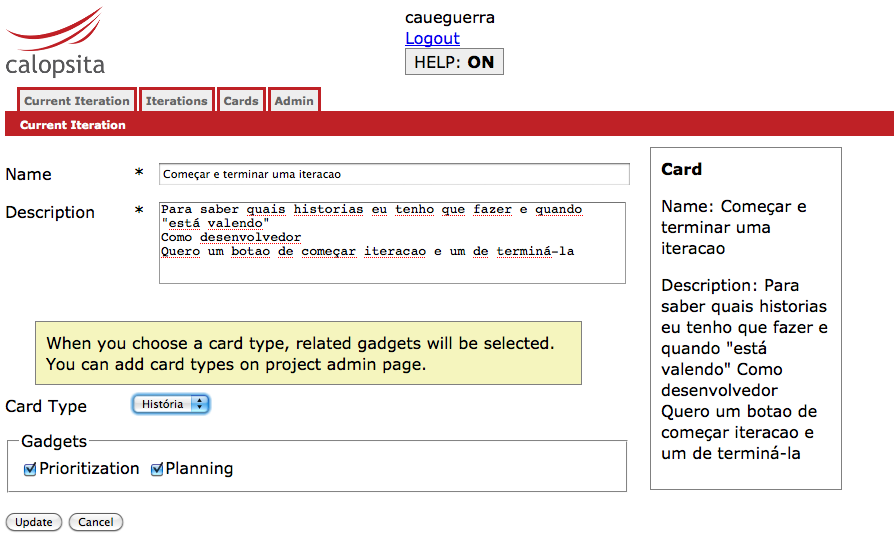
\includegraphics[width=110mm]{images/cartao.png}
  }
  \caption{Cartão}\label{figura:cartao}
\end{figure}

\subsubsection*{Tipos de Cartões}

Um tipo de cartão é, para o \calopsita{}, um agrupamento de \textit{gadgets} que definem o comportamento de um determinado cartão. Perceba que a noção é puramente semântica, já que os \textit{gadgets} podem ser habilitados e desabilitados individualmente, por cartão.

\begin{figure}[H]
  \centering
  \fbox{
    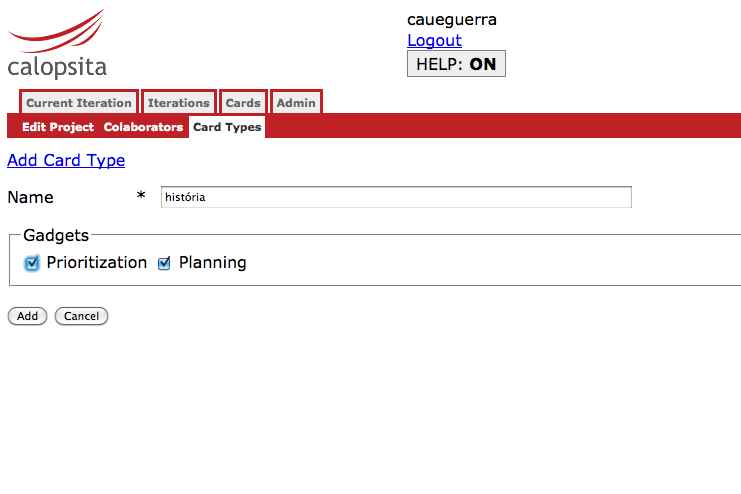
\includegraphics[width=110mm]{images/tipo_cartao.png}
  }
  \caption{Tipos de Cartões}\label{figura:tipo_cartao}
\end{figure}

\subsubsection*{Iterações}




Log, feed de mudanças

*****************
Falta coisa aqui... muita, btw
*****************

 

\subsection{Calopsita Plugins}

Como explicado anteriormente, o \calopsita{} possuí um núcleo com as funcionalidades essenciais e as demais serão fornecidas através de \textit{plugins}. Temos em nosso \textit{backlog}, diversos plugins para serem implementados e que já viriam na instalação padrão do \calopsita{}. Segue abaixo uma breve descrição de cada um deles:

\begin{itemize}
	\item{Priorização: permite seja atribuída uma prioridade a um determinado cartão através de uma interface baseada em \textit{drag 'n' drop}. Esse plugin já está implementado.
	
	\begin{figure}[H]
	  \centering
	  \fbox{
	    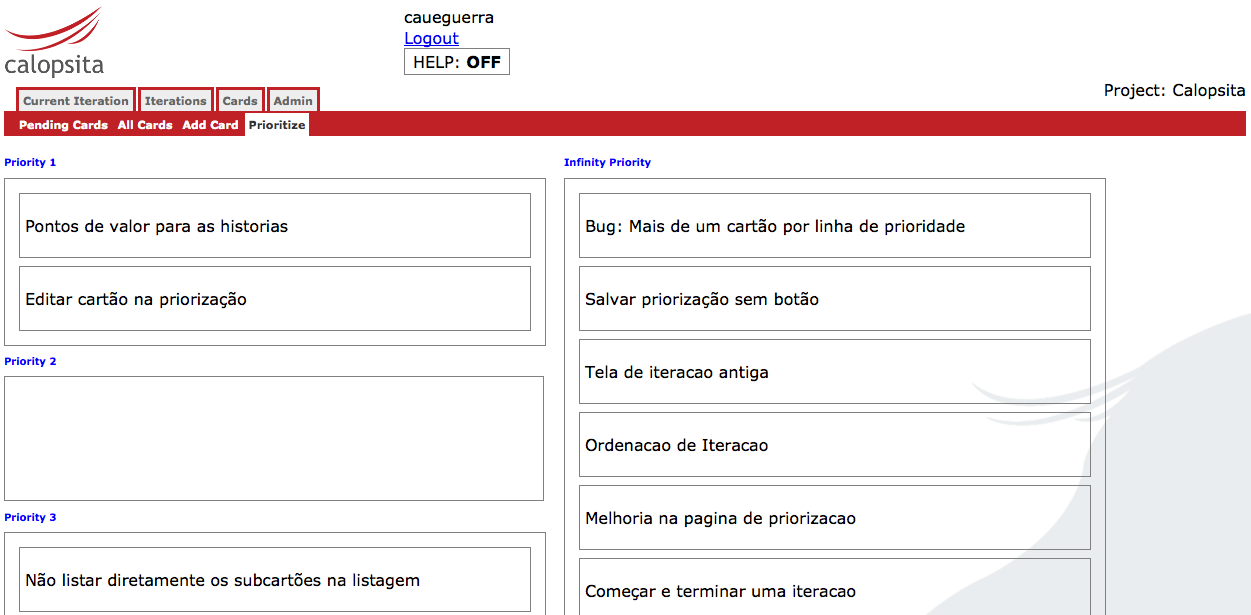
\includegraphics[width=110mm]{images/priorizacao.png}
	  }
	  \caption{Priorizacao}\label{figura:priorizacao}
	\end{figure}
	}
	\item{Planejamento: permite que cartões sejam adicionadas ou removidas de uma determinada iteração. Também baseado em \textit{drag 'n' drop} e já está implementado.
	
	\begin{figure}[H]
	  \centering
	  \fbox{
	    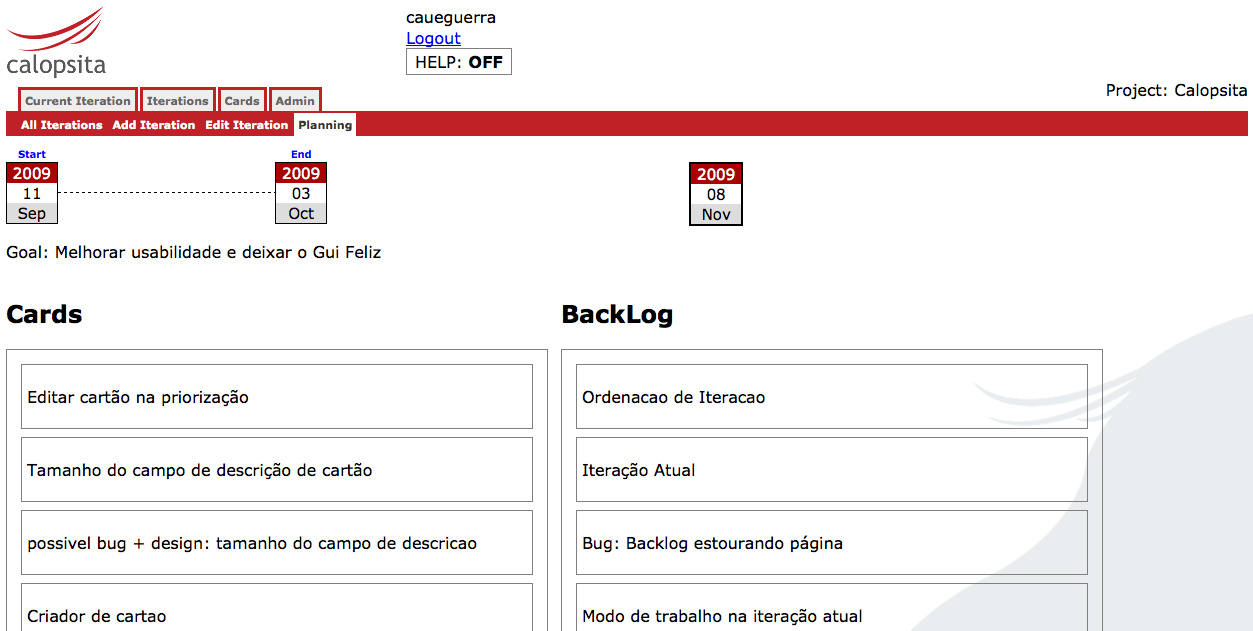
\includegraphics[width=110mm]{images/planejamento.png}
	  }
	  \caption{Planejamento}\label{figura:planejamento}
	\end{figure}
	}
	\item{Gráfico burn-up: a idéia desse plugin é que uma nova página contendo o gráfico burnup de uma determinada iteração sejá criada.}
	\item{Gráfico burn-down: a idéia desse plugin é que uma nova página contendo o gráfico burndown de uma determinada iteração sejá criada.}
	\item{Marcação de horas: esse plugin permitirá que a pessoa que trabalhou na conclusão de determinado cartão possa marcar o número de horas trabalhadas.}
	\item{Estimativas: possibilitará que um cartão tenha sua dificuldade estimada em pontos.}
	\item{Personas: criará uma área especial para a definição de personas. Essas personas poderão ser utilizadas mais facilmente na criação de novos cartões.}
	\item{Integração com GitHub: permitírá que comentários feitos no \textit{commit} do projeto no GitHub consigam mover cartões dentro de uma determinada iteração e mudar seu status.}
\end{itemize}
\section{Visão dos clientes e comparativos}

\subsection{Visão dos clientes}

Foi feita uma entrevista com nossos clientes onde questionamos suas expectativas, sobre o processo de desenvolvimento, e se o produto final satisfez o esperado.

Sobre a visão inicial, todos eles esperavam de alguma maneira um sistema que se pudesse de alguma forma substituir, na impossibilidade de uso, um quadro branco, ou ainda, substituir a ferramenta que vinham utilizando. 

Sobre o processo de desenvolvimento, gostaram do ritmo que o projeto teve, das personas que foram criadas, do deploy automatizado

Sobre o produto final, perguntamos se ele atendia a visão inicial, e disseram que embora a visão inicial tenha mudado muito, ficaram bastantes satisfeitos, mesmo reconhecendo que ainda há muita coisa a ser feita. Uma das frases que o Hugo citou em sua entrevista, vale a pena ser mencionada:

``A usabilidade é inquestionável, o \calopsita{} é um projeto que mostra CLARAMENTE uns 15 anos de avanço em cima do \textit{XPlanner} do ponto de vista da usabilidade.''

\subsection{Comparativo com outras ferramentas}

Antes de iniciar o desenvolvimen	to do \calopsita{}, analisou-se outras alternativas de proposta semelhante disponíveis no mercado. Uma análise bem extensa foi feita, tanto de produtos pagos, quanto de gratuitos e \opensource{}. A intenção é descobrir quais os pontos fortes de cada ferramenta e implementá-los no \calopsita{}. 

Embora as ferramentas pagas não sejam exatamente concorrentes, dado o grande investimento que é feito nelas, mostrar que o sistema desenvolvido tem as mesmas ou mais funcionalidades que as alternativas pagas pode fazer com que mais usuários e colaboradores sejam atraídos.

\begin{itemize}
\item{\textbf{Scrumy - https://scrumy.com/}

É uma ferramenta paga e proprietária, com uma interface baseada em \textit{drag 'n' drop}. Não permite nenhum tipo de personalização, nem estimativas, marcação de horas, uso de \textit{templates} ou \textit{personas}. Quanto aos gráficos, o único disponibilizado é o \textit{burndown}. 

Como diferencial, permite a visualização do projeto em algum ponto do passado, atualizando o kanban para representar o estado do projeto naquele ponto, além de permitir atualizações automáticas, ou seja, caso dois usuários estejam mexendo nele ao mesmo tempo, um enxerga as alterações do outro sem precisar recarregar a página.}

\item{\textbf{ScrumNinja - http://scrumninja.com}

É uma ferramenta paga e proprietária, bem pouco personalizável, sem a possibilidade de marcação de horas nem de trabalhar com \textit{templates} ou \textit{personas}. Tem suporte a estimativas, uma interface baseada em estados (start, deliver, etc) e gráficos de progresso. 

Um diferencial está no fato de que possui uma API que pode ser utilizada para a atualização dos cartões.}

\item{\textbf{Scrum'd - http://scrumd.com/}

É uma ferramenta paga e proprietária, não personalizável, que permite a estimativa de histórias em pontos e de tarefas em horas. Faz uso de \textit{burndown} e não trabalha com \textit{templates} nem \textit{personas}. 

Como diferencial, permite a importação e exportação de tarefas e histórias.}

\item{\textbf{Pivotal Tracker - http://www.pivotaltracker.com/}

É uma ferramenta proprietária, porém gratuita, que permite a estimativa de histórias em pontos e a marcação da velocidade do time. Também não trabalha com \textit{templates} nem \textit{personas}. 

Como diferencial permite a importação e exportação de tarefas e histórias, assim como permite a classificação de uma história em \textit{bug/feature/chore/release}.}

\item{\textbf{XPlanner - xplanner.org/}

É uma ferramenta livre e \opensource{}, que vem sendo utilizada pela disciplina de Programação Extrema na USP. Ele tem muitas funcionalidades, no entanto sua interface de uso não é das mais agradáveis. O uso do XPlanner por todos do time foi também um fator motivador na criação do \calopsita{}. Esse sistema não é personalizável nem trabalha com \textit{templates} ou \textit{personas}.

Quanto aos seus pontos positivos, o XPlanner permite o uso de estimativas e marcação de horas.}

\item{\textbf{VersionOne - http://www.versionone.com}

Ferramenta paga  e proprietária, personalizável e com suporte a marcação de velocidade, geração de \textit{burndown}. Não trabalha com \textit{templates} nem \textit{personas}.

Tem como diferencial a possibilidade de planejamento de releases. É a única ferramenta analisada com suporte a diferentes metodologias.}

\item{\textbf{Pronto - http://www.bluesoft.com.br/pronto-demo}

Ferramenta \opensource{} e brasileira. Permite a marcação de horas trabalhadas, bem como a geração de gráficos (embora, durante os testes, a geração de \textit{burndowns} tenha apresentado problemas). Não permite customizações nem o uso de \textit{templates} ou \textit{personas}. 

Como diferencial permite que usuários tenham perfis diferentes (\textit{product owner}, \textit{scrum master}, desenvolvedor, testador, etc) e permite informar se a tarefa for concluída usando pareamento, apontando a dupla envolvida.}

\item{\textbf{PPTS - http://ses-ppts.sourceforge.net/}

É uma ferramenta \opensource{} que possibilita a priorização de tarefas, bem como permite saber quais pessoas estiveram envolvidas em quais tarefas. Permite a geração de gráficos diversos, bem como a estimativa de tarefas e a geração de relatório com a velocidade do time. 

Como diferencial, permite a customização de menus.}

\item{\textbf{Rally - http://www.rallydev.com/}

Ferramenta proprietária, que permite a customização por widgets e usuários com diferentes perfis. 

Um diferencial está no fato de que permite integração com a IDE Eclipse.}

\item{\textbf{Mingle - http://studios.thoughtworks.com/mingle-agile-project-management}

Ferramenta proprietária que conta com a geração de gráficos, estimativas, priorização, marcação de horas. Permite uma certa customização, mas não permite o uso de \textit{templates} nem de \textit{personas}. 

Como ponto positivo, está o fato de que se adapta a diferentes metodologias ágeis e possui integração com o \textit{Google Wave}.}

\end{itemize}

\subsection{Quadro comparativo}

No quadro comparativo a seguir pode-se visualizar de maneira mais simples quais ferramentas têm e quais não têm algumas características levantadas como importantes para a equipe do \calopsita{}. 

\begin{tabular}{|l|l|l|l|l|l|l|l|l|l|l|}
	\hline
	\multicolumn{11}{|c|}{Aplicações similares} \\
	\hline
	                & A & B & C & D & E & F & G & H & I & J \\
	Calopsita       & X & X & X & X & X & * & X & * & X & * \\
	Scrumy          & - & - & - & X & X & - & - & - & - & - \\
	ScrumNinja      & - & - & X & X & X & - & X & - & - & - \\
	Scrum'd         & - & - & X & X & X & - & X & - & - & - \\
	Pivotal Tracker & X & - & X & X & X & X & X & - & - & - \\
	XPlanner        & X & X & - & X & X & X & X & - & - & - \\
	VersionOne      & - & - & X & X & X & X & X & X & - & - \\
	Pronto          & X & X & - & X & X & X & - & - & - & - \\
	PPTS            & X & X & X & X & X & X & X & - & - & - \\
	Rally           & - & - & X & X & X & X & X & - & - & - \\
	Mingle          & - & - & X & X & X & X & X & X & - & - \\
	\hline
	\multicolumn{11}{l}{\textbf{Legenda:}} \\
	\multicolumn{4}{l}{A - Gratuito} & \multicolumn{7}{l}{F - Marcação de horas} \\
	\multicolumn{4}{l}{B - Opensource} & \multicolumn{7}{l}{G - Estimativas} \\
	\multicolumn{4}{l}{C - Personalizável} & \multicolumn{7}{l}{H - \textit{Templates} de metodologias} \\
	\multicolumn{4}{l}{D - Gráficos} & \multicolumn{7}{l}{I - \textit{Templates} de cartões} \\
	\multicolumn{4}{l}{E - Priorização} & \multicolumn{7}{l}{J - \textit{Personas}} \\
	\multicolumn{11}{l}{* - no \textit{backlog} para ser feito} \\
\end{tabular}

\section{Conclusão}

Embora já esteja sendo utilizado há 6 meses em projetos pessoais e comerciais, não apenas pela equipe, mas também por outras equipes e desenvolvedores, o \calopsita{} ainda tem muito para onde crescer -- e é intenção que o projeto cresça.

O plano para o próximo ano é que mais empresas adotem o \calopsita{} para o gerenciamento de suas aplicações. Para esse objetivo, há um trabalho de divulgação da solução para diversos grupos de desenvolvimento de grandes empresas que já utilizam métodos ágeis.

Além disso, o \calopsita{} será um dos projetos desenvolvidos na matéria de programação extrema no próximo semestre do IME. Com isso, além de continuar o desenvolvimento do projeto, pretende-se colocar os alunos em contato com diferentes métodos e \textit{frameworks} adotados no mundo.

Entre os ítens de maior valor para os clientes, os seguintes \textit{plugins} serão implementados muito em breve:

\begin{itemize}
	\item{Ordem de cartões: cartões de uma mesma prioridade devem poder ter precedência sobre outros de uma mesma iteração;}
	\item{Gráfico de burnup: para marcar o andamento de uma iteração, um gráfico de acompanhamento das tarefas prontas no decorrer do tempo.}
	\item{Kanban: o quadro branco usado por diversas metodologias para manter a equipe informada do que acontece no projeto.}
\end{itemize}

A respeito do que foi desenvolvido durante todo o ano e do suporte que a equipe recebeu das muitas pessoas que se envolveram no projeto, muitos agradecimentos devem ser feitos. Em particular, à Mariana Bravo, ao Hugo Corbucci, ao orientador Alfredo Goldman, ao Guilherme Silveira e aos demais profissionais da Caelum que enriqueceram o \calopsita{} com valiosas opiniões. 

No geral, há uma satisfação da equipe com o que foi desenvolvido, não só no sistema entregue, mas também no ferramental de suporte -- os outros projetos \opensource com os quais colaboramos para que se adequassem às necessidades do \calopsita{}.

E é com esse espírito de colaboração do \opensource que contamos para o sucesso do projeto. Com a facilidade de criação de \textit{plugins} e as muitas necessidades específicas de cada time, a equipe está esperançosa na multiplicação das extensões do \calopsita{}.

No mais, foi um prazer desenvolver um projeto de utilidade para a comunidade ágil e aprender as tantas diferentes tecnologias e métodos que se estudou durante a construção do \calopsita{}. E essa construção só foi possível somando-se o que foi aprendido no curso com o conhecimento adquirido no estágio.

\section{Bibliografia}

\begin{thebibliography}{30} 

\bibitem{po} http://www.scrumalliance.org/articles/44-being-an-effective-product-owner
\bibitem{scrum} Ken Schwaber (2004). \textit{Agile Project Management with Scrum}. Microsoft Press.
\bibitem{xp} Kent Beck (2004). \textit{Extreme Programming Explained}. Addison-Wesley; 2nd edition
\bibitem{kanban} http://www.infoq.com/articles/agile-kanban-boards
\bibitem{brooks} Frederich Brooks (2010). \textit{Design of Design}. Addison-Wesley Professional; 1st edition
\bibitem{manifesto} Kent Beck, Alistair Cockburn, Martin Fowler, et al. \textit{Agile Manifesto}. http://www.agilemanifesto.org;
\bibitem{waterfall} Winston W Royce (1970). \textit{Managing the development of large software systems}.
Proceedings of IEEE Wescon, 1970;
\bibitem{rup} Rational Software Corporation (2000). \textit{Rational Unified Process -- Best Practices for Software Development Teams}. White paper;
\bibitem{pair} Laurie Williams, Alistais Cockburn (2001). \textit{The costs and benefits of pair programming}. Extreme programming examined, 2001 - Citeseer;
\bibitem{refactoring} Martin Fowler, Kent Beck, et al (1999). \textit{Refactoring: Improving the Design of Existing Code}; 1st edition;
\bibitem{ci} http://martinfowler.com/articles/continuousIntegration.html(2006)
\bibitem{dsl} http://martinfowler.com/bliki/DomainSpecificLanguage.html (2006)
\bibitem{di} http://www.informit.com/articles/article.aspx?p=1404056 (2009)
\bibitem{fowler} Martin Fowler (2002). \textit{Patterns of Enterprise Application Architecture}.  Addison-Wesley Longman Publishing Co., Inc.
\bibitem{dao} http://java.sun.com/blueprints/corej2eepatterns/Patterns/DataAccessObject.html
\bibitem{rest} Leonard Richardson, Sam Ruby (2007). \textit{RESTful Web Services}. O'Reilly
\bibitem{gof} Erich Gamma, Richard Helm, Ralph Johnson, John Vlissides J (1995). \textit{Design Patterns: Elements of reusable object-oriented software}. Addison-Wesley, 1st edition
\bibitem{effective} Joshua Bloch (2008). \textit{Effective Java}. Addison-Wesley; 2nd edition
\bibitem{rest-jim} http://jim.webber.name/downloads/presentations/2009-05-HATEOAS.pdf
\bibitem{ddd} Eric Evans (2004). \textit{Domain Driven Design}. Addison-Wesley; 1st edition 
\bibitem{rest-roy} Roy Fielding (2000). \textit{Architectural Styles and the Design of Network-based Software Architectures}. http://www.ics.uci.edu/~fielding/pubs/dissertation/top.htm
\bibitem{rest-infoq} http://www.infoq.com/articles/rest-introduction
\bibitem{mimetypes} http://www.iana.org/assignments/media-types/
\bibitem{bdd} Dan North (2006). http://dannorth.net/introducing-bdd

\end{thebibliography}

\newpage
\section{Apêndice I - Personas}
\label{sec:personas}

\begin{itemize}
	\item{Olivia (desenvolvedora)
	
	``Eu tenho que usar esse sistema... mas o que eu quero MESMO é que ele não atrapalhe meu
	trabalho''.
	
	Se fosse por ela, ela usava quadros na parede. Mas como sua equipe (inclusive cliente) não trabalha num mesmo ambiente físico, eles precisam usar o \calopsita.}
	\item{Nano (desenvolvedor remoto)
	
	``Quero saber o que já foi feito e qual é a próxima tarefa que eu tenho que fazer''.
	
	Nano mora no Havaí e trabalha com uma equipe no Brasil.}
	\item{Morelli (cliente)
	
	``Quero saber como anda o desenvolvimento da minha grande ideia''. 
	
	Morelli é um cliente que não sabe nada sobre desenvolvimento de software com uma grande ideia de um software para seu negócio.}
	\item{Fabs (colaborador distraído)
	
	``Eu quero bater o olho na página... e obter a informação que eu preciso''.
	
	Fabs algumas vezes é cliente, outras vezes é desenvolvedor. Sempre tem muitas coisas para fazer e não presta muita atenção em nada.}
	\item{Vinicius (\textit{coach} XP)
	
	``Quero ter uma visão geral do meu projeto XP''.}
	\item{Alexandre (\textit{scrum master})
	
	``Quero gerenciar meus projetos Scrum com facilidade''.}
	\item{Daniel (usuário leigo)
	
	``Muito legal esse negócio, mas como usa?''. 
	
	Daniel acaba de entrar num curso de computação e ouviu seus veteranos falando do \calopsita{}. Ele não sabe muita coisa de desenvolvimento, muito menos de métodos ágeis. Na verdade, ele mal sabe usar o computador mas é empolgado e quer aprender e ninguém pode ajudar.}
\end{itemize}

\newpage
\section{Apêndice II - Criando plugins}

A criação de plugins no calopsita é baseada em pontos de extensão. Os pontos de extensão já implementados são:

\begin{itemize}
	\item{\textbf{Gadget} - Implemente uma entidade do Hibernate com essa interface, e então você pode adicionar informações
		aos cartões que possuirem esse gadget. Por exemplo se você quiser adicionar uma estimativa de velocidade, tempo total 
		ou dificuldade do cartão}
	\item{\textbf{Transformer} - Implemente essa interface e anote a classe gerada com @Component. Assim você consegue
		modificar as listagens, por exemplo mudando a ordenação ou removendo determinados itens.}
	\item{\textbf{PluginConfig} - Implemente essa interface e anote a classe gerada com @Component. Com ela é possível
		adicionar itens aos menus do sistema, baseados nos parâmetros da requisição}
\end{itemize}

Além disso, você pode criar novas telas para o sistema. Para isso basta criar um controlador do 
VRaptor~\footnote{http://vraptor.caelum.com.br/documentacao} e as respectivas jsps de resultado.
Todas as classes geradas precisam estar abaixo do pacote \textbf{br.com.caelum.calopsita} para que o
VRaptor consiga enxergá-las.

Por exemplo, se fôssemos fazer um plugin para estimar velocidade dos cartões, precisamos criar as classes:

\begin{itemize}
	\item{o Gadget para adicionar informação ao cartão:
		\begin{lstlisting}
			package br.com.caelum.calopsita.plugins.velocidade;
			
			@Entity
			public class VelocidadeCard implements Gadget {
				@Id
				@GeneratedValue
				private Long id; // o id do banco
				
				@OneToOne
				private Card card; // o cartao que esse gadget vai adicionar informacao
				
				private Integer velocidade; // a informacao a mais
				
				// getters e setters
			}
		\end{lstlisting}	
	}
	\item{um Transformer para ordenar os cartões por velocidade:
		\begin{lstlisting}
			package br.com.caelum.calopsita.plugins.velocidade;
			@Component
			public class OrdenaPorVelocidadeTransformer implements Transformer<Card> {

				public boolean accepts(Class<?> type) {
					return type.equals(Card.class); // vai transformar listas de cartoes
				}

				public List<Card> transform(List<Card> list, Session session) {
					Collections.sort(list, new VelocidadeComparator()); // ordena a lista de acordo com o comparator abaixo
					return list;
				}

				public static class VelocidadeComparator implements Comparator<Card> {
					public int compare(Card esquerda, Card direita) {
						// pega o gadget do tipo dado do cartao. Null se o cartao nao tiver o gadget
						VelocidadeCard velocidadeEsquerda = esquerda.getGadget(VelocidadeCard.class); 
						VelocidadeCard velocidadeDireita = direita.getGadget(VelocidadeCard.class);
						
						// decide se o cartao da esquerda e maior que o da direita
						// de acordo com o contrato do comparator
						if (velocidadeEsquerda == null) {
							return 1;
						} else if (velocidadeDireita == null) {
							return -1;
						}
						return velocidadeEsquerda.getVelocidade() - velocidadeDireita.getVelocidade();
					}
				}
			}

		\end{lstlisting}
	}
	
	\item{um Controlador do VRaptor que vai tratar as requisições para esse plugin:
	
		\begin{lstlisting}
			package br.com.caelum.calopsita.plugins.velocidade;
			
			@Resource
			public class VelocidadeController {
				
				private Result result;
				public VelocidadeController(Result result) {
					this.result = result;
				}
				// seguindo o padrao das urls
				@Path("/projects/{project.id}/velocidade")
				@Get
				public List<Card> estima(Project project) {
					return project.getAllCards();
				}
	
				@Path("/projects/{velocidadeCard.card.project.id}/velocidade")
				@Post
				public void adiciona(VelocidadeCard velocidadeCard) {
					// salva o velocidadeCard no banco
					// redireciona para a estimativa de cartoes
					result.use(logic()).redirectTo(VelocidadeController.class).estima(velocidadeCard.getCard().getProject());
				}
				
			}
		\end{lstlisting}
	}
	
	\item{um jsp que responda mostre a tela de estimar cartões. Logo precisa estar em /WEB-INF/jsp/velocidade/estima.jsp
	\lstset{language=html,frame=ltrb,framesep=5pt,basicstyle=\footnotesize,
	  keywordstyle=\ttfamily\color{OliveGreen},
	 identifierstyle=\ttfamily\color{CadetBlue}\bfseries, 
	 commentstyle=\color{Brown},
	 stringstyle=\ttfamily,
	 showstringspaces=false,
	 showspaces=false,
	 tabsize=2}
	
		\begin{lstlisting}
			<!-- estilo da pagina, organizacao e etc -->
			<c:forEach items="${cardList}" var="card">
				<form action="<c:url value="/projects/${project.id}/velocidade" method="POST">
					<!-- campos do formulario passar valores para a logica -->
				</form>"
			</c:forEach>
		\end{lstlisting}
	}
\end{itemize}

Para instalar o plugin, basta colocar as classes criadas no classpath (dentro de um jar, ou no WEB-INF/classes),
jsps na pasta /WEB-INF/jsp, e eventuais javascripts e css's na pasta web.




\end{document}
